\section{Inledning}
Systemet består av en robot och tillhörande mjukvara. I detta dokument beskrivs hur roboten ska byggas. Detta dokument kan ses som en påbyggnad på systemskissen, som ger en översiktlig beskrivning av delsystemen. Designspecifikationen ska ge en mer detaljerad bild, dels av hur enheterna ska byggas var för sig och dels hur de ska synkroniseras för att tillsammans fungera som en större enhet.
Roboten kommer att bestå av tre enheter, vardera innehållandes en processor, som kan kommunicera med varandra. 
Enheterna kommer att monteras på en plattform med två drivande hjul och ett stödhjul samt tillhörande motorer.
Mjukvaran är avsedd för att köras på en PC och används för att kommunicera med roboten. 

\begin{figure}[H]
\centering
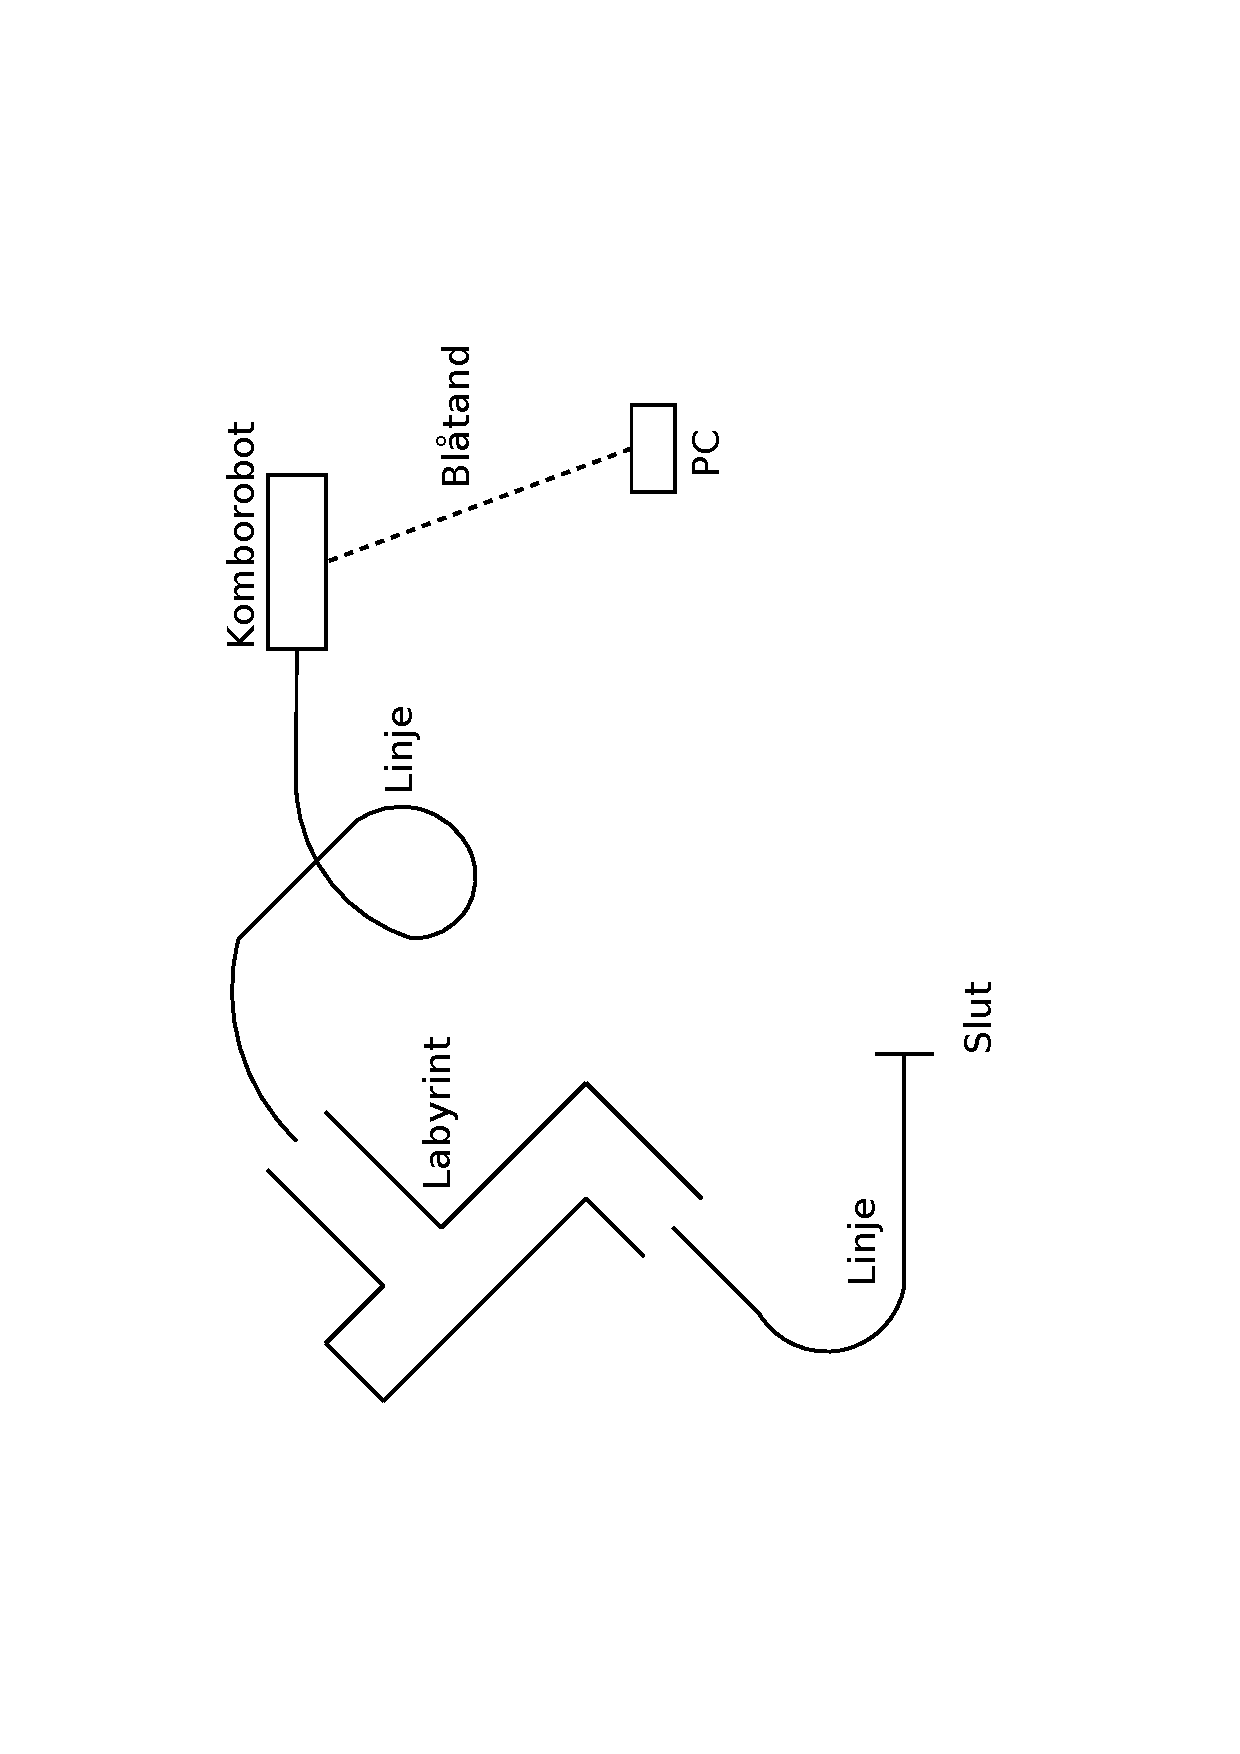
\includegraphics[angle=270,scale=0.5]{bilder/Oversikt.pdf}
\end{figure}
